The EASYGO project (\url{www.easygo-itn.eu}) has received funding from the European Union’s Horizon 2020 Research and Innovation Programme under the Marie Skłodowska-Curie Grant Agreement No 956965.

\begin{figure}
    \centering
    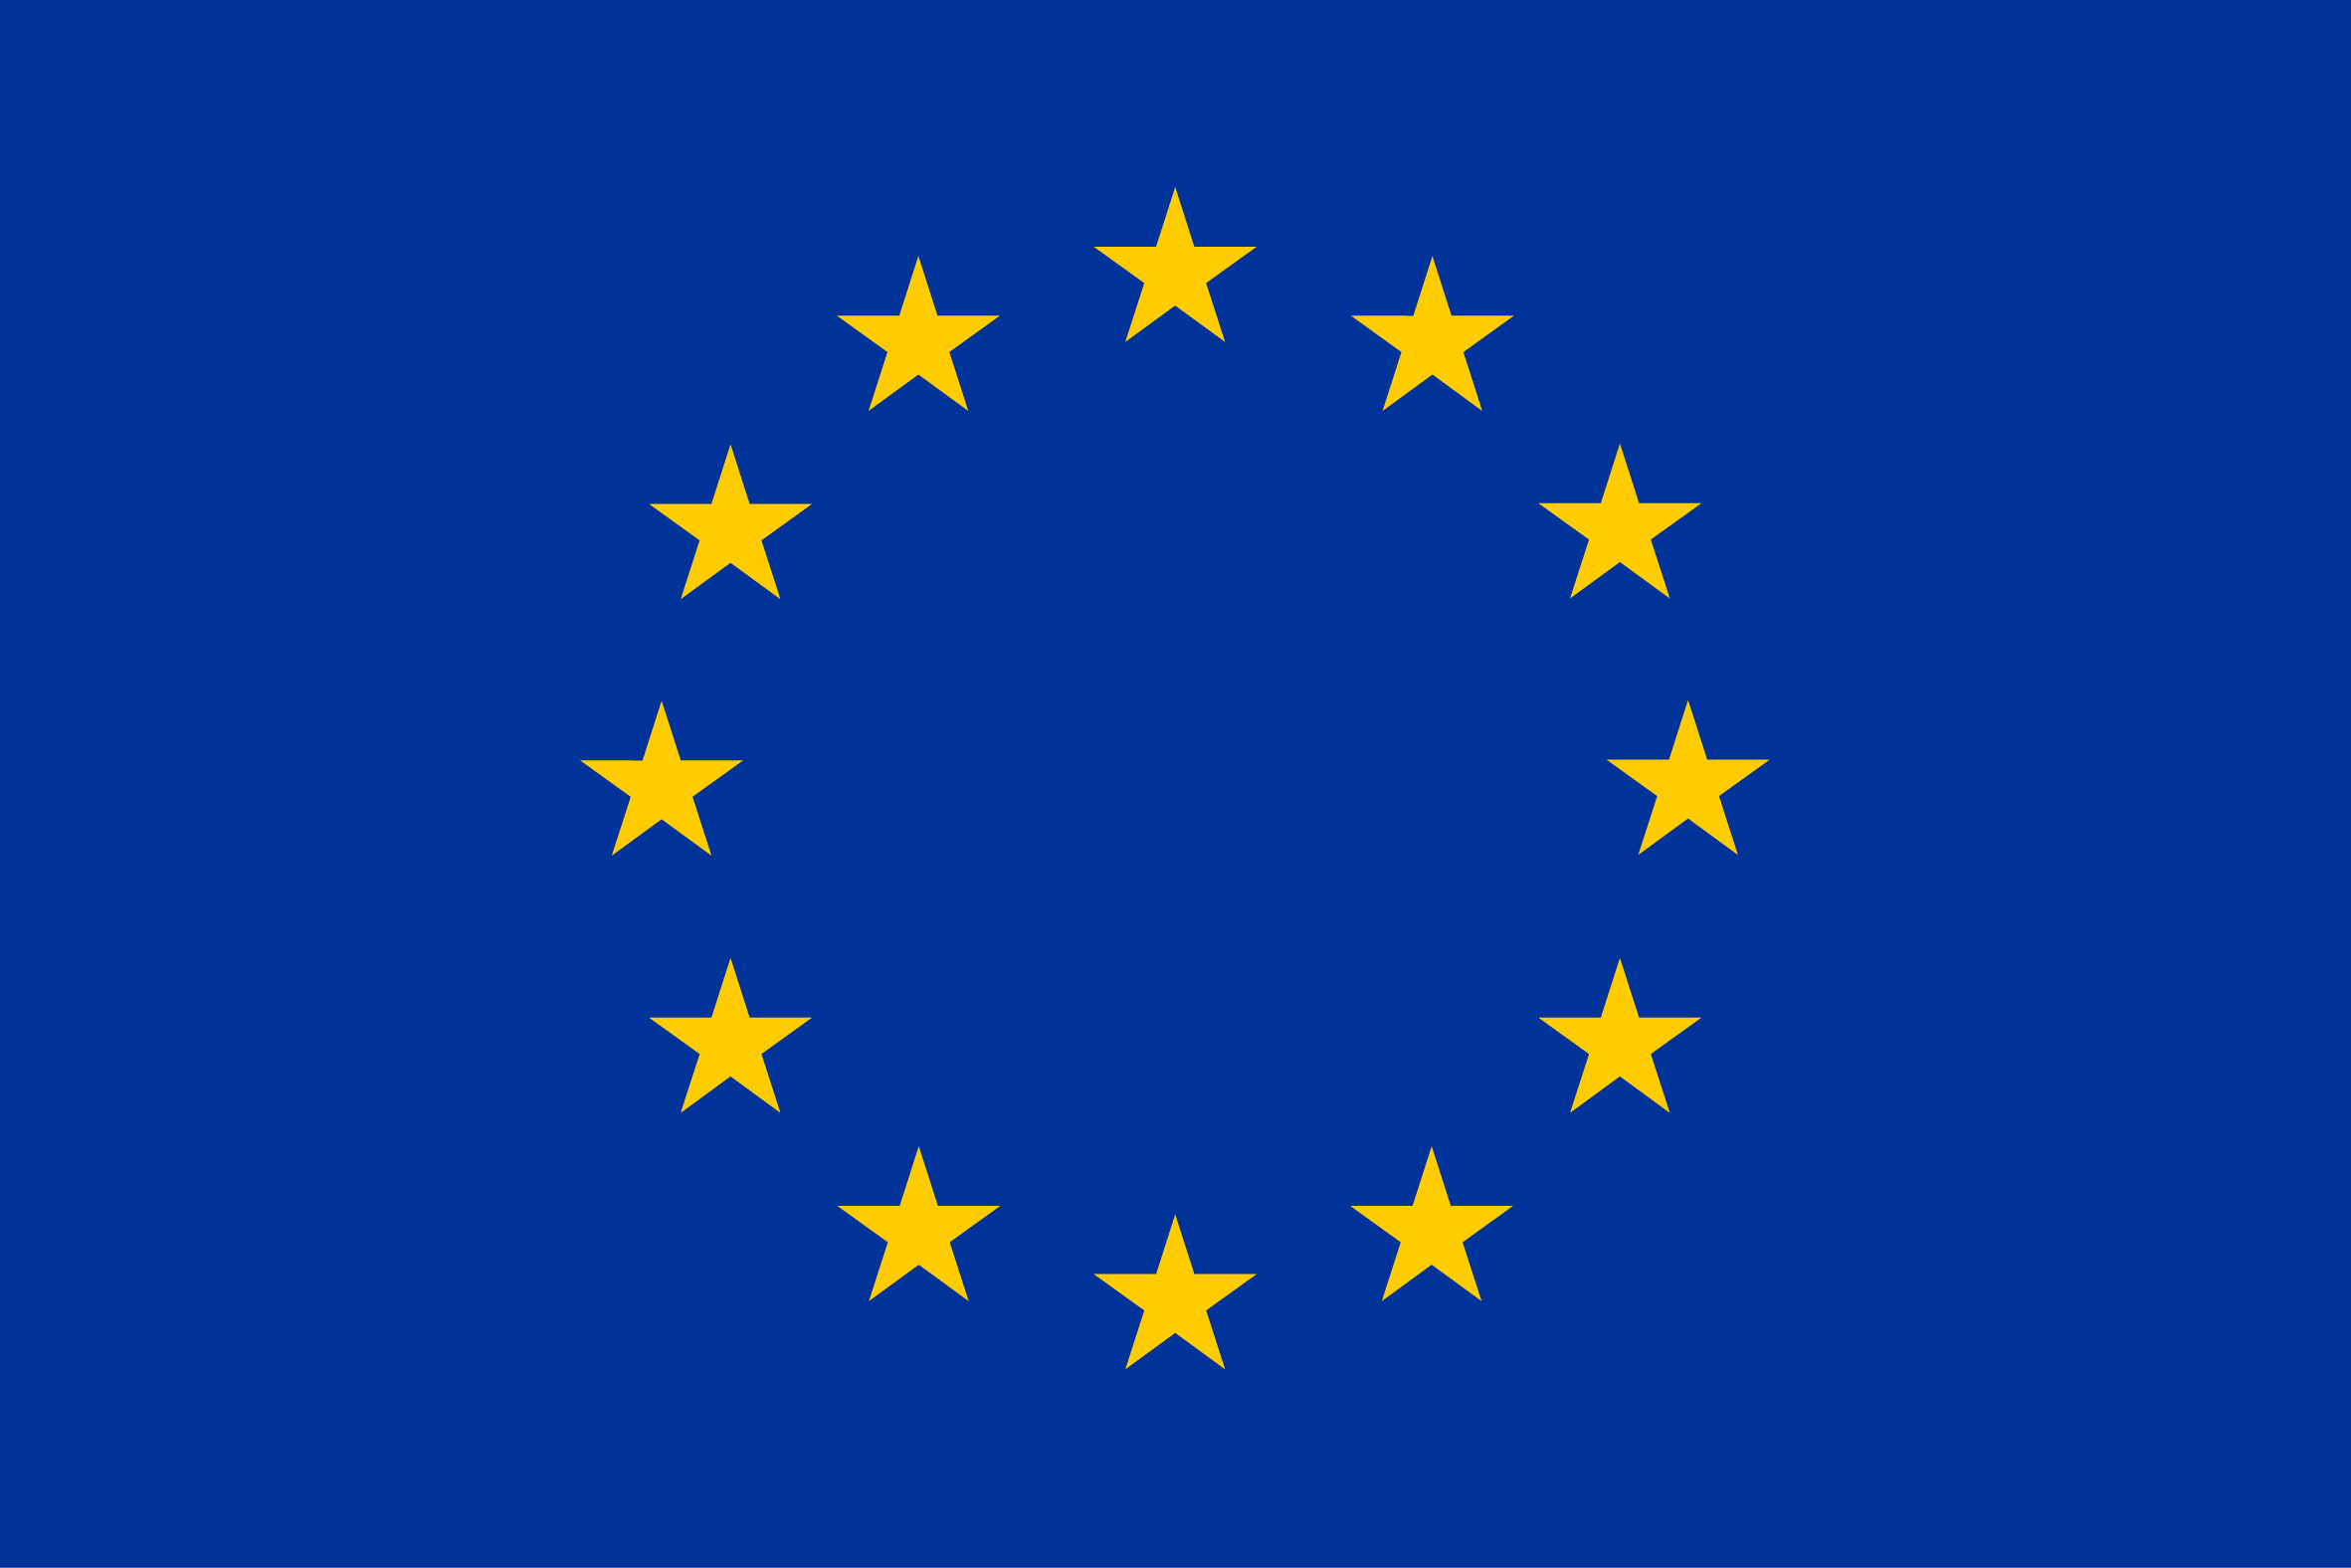
\includegraphics[width=0.25\linewidth]{Images/eu_logo.png}
    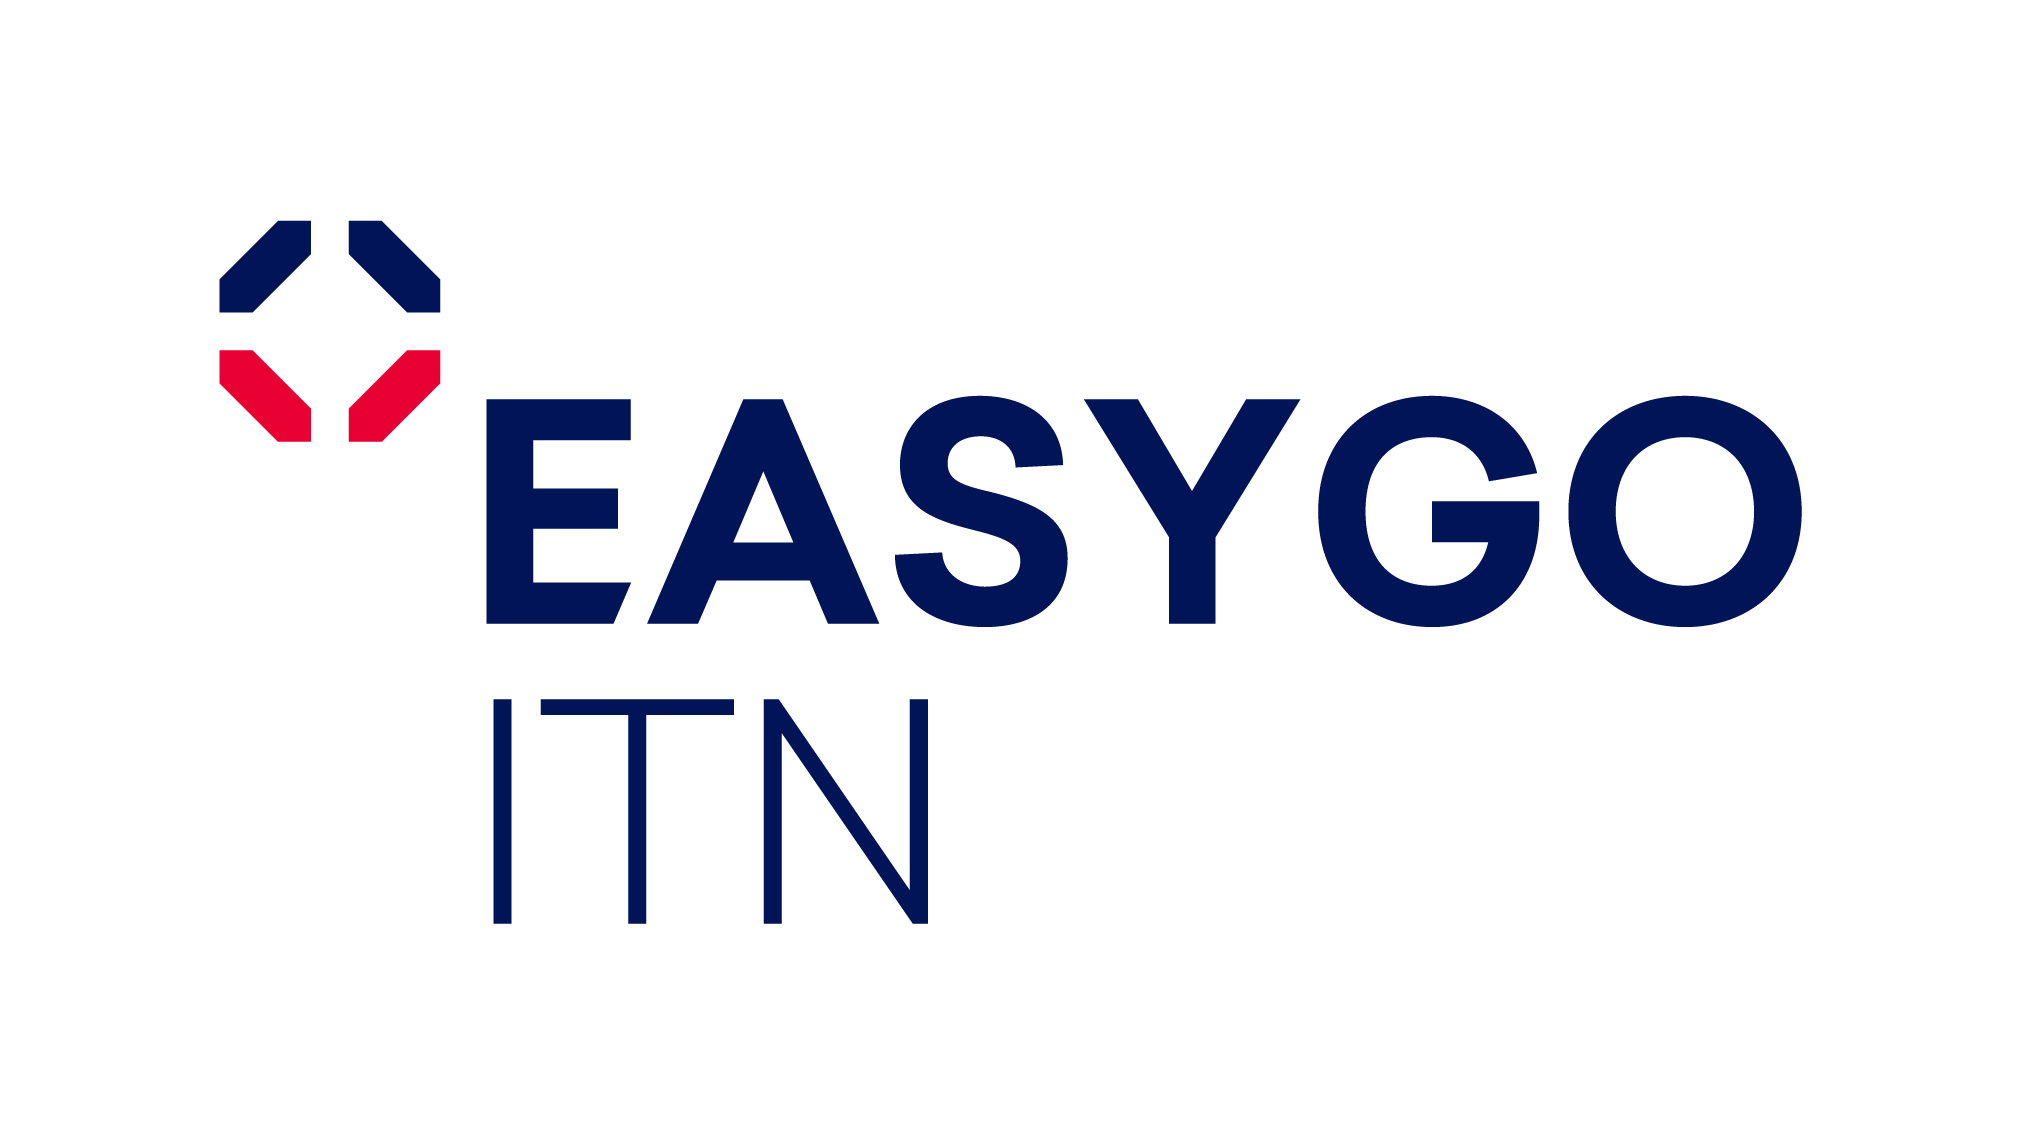
\includegraphics[width=0.25\linewidth]{Images/Logo-EasyGo-Color.png}
\end{figure}

A.M.M Leal and M.O Saar thank the Werner Siemens Foundation (Werner Siemens-Stiftung) for its support of the Geothermal Energy and Geofluids (geg.ethz.ch) Group at ETH Zurich, Switzerland, as well as the Energi Simulation Foundation (energisimulation.com) for partial funding of this research.

The contributions by D. Alfani were carried out within the NEST - Network 4 Energy Sustainable Transition (D.D. 1243 02/08/2022, PE00000021) and received funding under the National Recovery and Resilience Plan (NRRP), Mission 4 Component 2 Investment 1.3, funded from the European Union - NextGenerationEU. This manuscript reflects only the authors’ views and opinions, neither the European Union nor the European Commission can be considered responsible for them.
